% !TEX root = acl_latex.tex
% This must be in the first 5 lines to tell arXiv to use pdfLaTeX, which is strongly recommended.
\pdfoutput=1
% In particular, the hyperref package requires pdfLaTeX in order to break URLs across lines.
\documentclass[11pt]{article}
% Change "review" to "final" to generate the final (sometimes called camera-ready) version.
% Change to "preprint" to generate a non-anonymous version with page numbers.
\usepackage[final]{acl}
% Standard package includes
\usepackage{times}
\usepackage{latexsym}
% For proper rendering and hyphenation of words containing Latin characters (including in bib files)
\usepackage[T1]{fontenc}
% For Vietnamese characters
% \usepackage[T5]{fontenc}
% See https://www.latex-project.org/help/documentation/encguide.pdf for other character sets
% This assumes your files are encoded as UTF8
\usepackage[utf8]{inputenc}
% This is not strictly necessary, and may be commented out,
% but it will improve the layout of the manuscript,
% and will typically save some space.
\usepackage{microtype}
% This is also not strictly necessary, and may be commented out.
% However, it will improve the aesthetics of text in
% the typewriter font.
\usepackage{inconsolata}
%Including images in your LaTeX document requires adding
%additional package(s)
\usepackage{graphicx}
% To be able to comment out blocks of text
\usepackage{comment}
% To be able to use colors
\usepackage{xcolor}

\usepackage{float}

\title{Evaluation of Named Entity Recognition in \\ Latin using an Unsupervised Model}


\author{
  Gabriel Cristian Circiu \\
  IT University of Copenhagen \\ Copenhagen, Denmark \\
  \texttt{gaci@itu.dk} \\\And
  Mykyta Taranov \\
  IT University of Copenhagen \\ Copenhagen, Denmark \\
  \texttt{myta@itu.dk} \\\And
  Wenzel Keil \\
  IT University of Copenhagen \\ Copenhagen, Denmark \\
  \texttt{weke@itu.dk}
}

\begin{document}
\maketitle
\begin{abstract}
Tackling the challenges of Natural Language Processing (NLP) in Latin using an unsupervied model has lead to the observation that certain tokenizers 
such as BERT are better suited for such tasks and that the choice of the model itself plays a significant role in the final results.
Clustering has proved to be the most straight-forward method to group entities together but a more intricate pipeline lead to a significantly 
better result, achieving an averaged macro F1 score of 0,51.
\end{abstract}

\section{Introduction}

As international students, the probability of sharing a common language outside of English is not high, however, during our studies we came to the 
realization that some of usshare knowledge in one such language, Latin. Albeit we are nowhere near fluent, it has sparked curiosity to work with it.
We chose to head in the direction of our shared curiosity of Latin, and to poke at it within the Named Entity Recognition (NER) sphere.

As such we chose to build upon a past research, titled 
\textit{Challenges and Solutions for Latin Named Entity Recognition}\footnote{Original paper: \url{https://aclanthology.org/W16-4012/}}
\cite{erdmann-etal-2016-challenges}, which tackles the problem of NER in Latin using a supervised and semi-supervised model.
Our dataset is based on the one used in the original paper, following the same structure, with some additional specifications for clarity.

\section{Dataset}

The dataset from the original paper named 3 works of literature, Caesar's \textit{De Bello Gallico (BG)}, Pliny the Younger's \textit{Epistulae (EP)},
and Ovid's \textit{Ars Amatoria (AA)}. We have had the great fortune of receiving the full dataset in its entirety, as large text files, in IOB format.
While all the literature was scrambled in each file, having it in the right format has made it all the more easier to process, and do some
Exploratory Data Analysis (EDA). After thorough investigation, we have found that there is a slight inconsistency in the original paper regarding 
the dataset, and that of which we have received. As mentioned, the entirety of \textit{BG}, and parts of \textit{EP} and \textit{AA} were annotated,
however, parts of Caesar's \textit{De Bello Civili (BC)} were also annotated within the dataset, but left unmentioned in the original paper.

To have an initial understanding of the expectations of our models, we must understand the distribution of the dataset, namely the amount of
\textit{Named entities (NE)} and \textit{Non-Named entities (Non NE)} in the dataset. As shown in Figure~\ref{fig:NER-Train} and Figure~\ref{fig:NER-Test}, 
we can see that there is a significant imbalance in the dataset, with only about 5.5\% and 3.3\% of the tokens being NE.

\begin{figure}[H]
  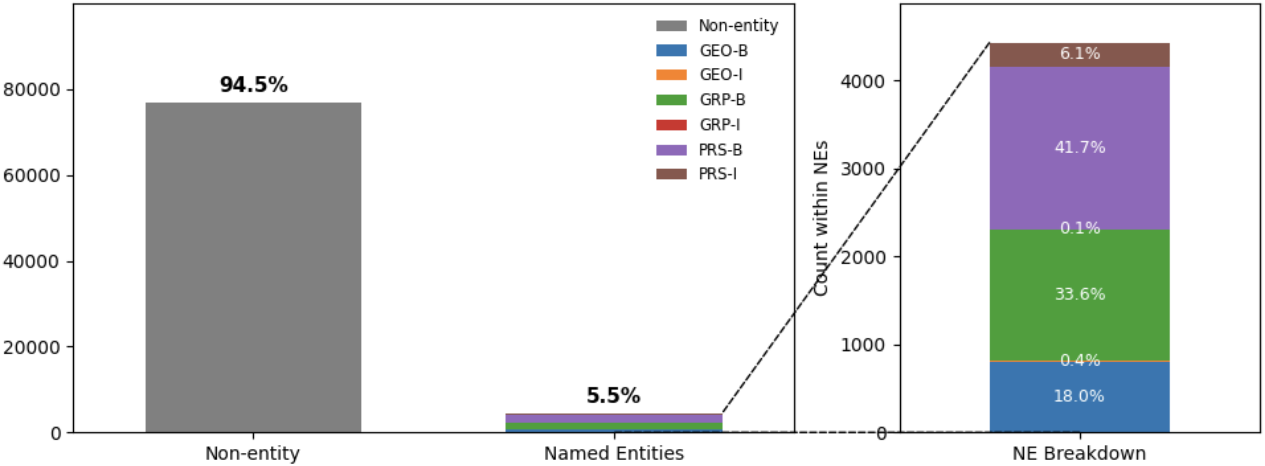
\includegraphics[width=\columnwidth]{NER-Train.png}
  \caption{Distribution of data for \textit{BG}, \textit{BC}, and \textit{AA} combined, used for one of the training folds.}
  \label{fig:NER-Train}
\end{figure}

\begin{figure}[H]
  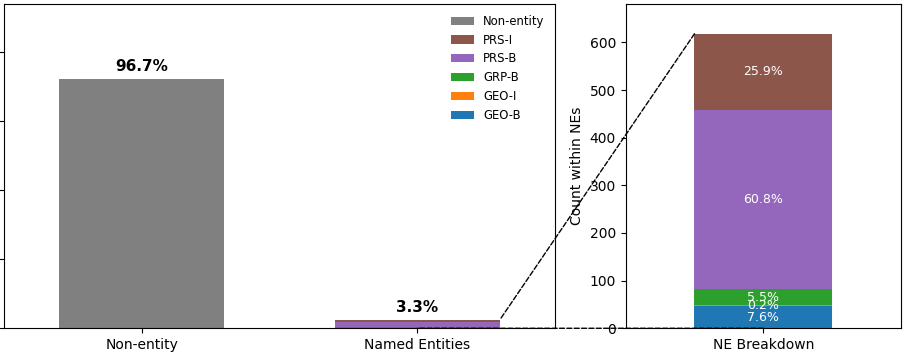
\includegraphics[width=\columnwidth]{NER-Test.png}
  \caption{Distribution of data for \textit{EP}, used for one of the testing folds.}
  \label{fig:NER-Test}
\end{figure}

\section{Methodology}

Once we had the dataset split into training and testing files, we started with tokenizing the words, and finding a solutions on how to
handle the words, embeddings, and labels, without having supervision over the original labels that we were given. Afterwards we have decided on
multiple approaches in training a model, namely Clustering, and a Neural Network.

\subsection{Embeddings}

Our initial approach was to vectorize tokens using a basic \texttt{Word2Vec} method from the \texttt{Gensim} library. However, this produced 
unacceptably low results with clustering — the model wasn’t able to separate entities from non-entities in a meaningful way. So we moved on to
a more powerful method: using contextual word embeddings from a \texttt{pretrained Bidirectional encoder representations from transformers (BERT)} model,
specifically \texttt{bert-base-multilingual-cased}. This model was trained on a large corpus of multilingual text, including Latin, and is
capable of generating high-quality embeddings for words in context.

We used the \texttt{Hugging Face Transformers} library to load the model and generate embeddings for our tokens. We extacted the embeddings
from the last hidden layer of the model. Since \texttt{BERT} works on subword level, we combined the embeddings of the subwords that make up
a token by averaging subwords embeddings. This approach has been shown to work well in practice and allows us to obtain a single embedding for
each token. We discusse the options of using subwords embeddings for clustering and switching to the word level later on, but this led to
unnecessary complications of the pipeline, for example, by introducing the necessaty of handling scenarios when embeddings of one word end up
in different clusters.

\subsection{Clustering}

Once we had the word level embeddings, we applied \texttt{KMeans Clustering} to automatically group the tokens into clusters. \texttt{Kmeans}
was the most straightforward choice for the task. One of the challenges we faced was the choice of \texttt{K} - number of clusters. We tried
several methods to determine the optimal number of clusters, including the \textit{Elbow Method} and \textit{Silhouette Score}. 
The elbow method suggested that big values of \texttt{K} are better, up to the point that number of clusters was close to the number of tokens.
Silhouette score also was not very helpful, since bigger score didn't correspond to better evaluation scores afterwards. So we boiled down the
problem to the simplest approach: trial and error.
First we started with a binary classification, where we had two clusters: one for NE and one for Non NE. For this we settled on a value of \texttt{K} = 7.500 
where we then passed the clusters classified as NE to another kmeans clustering, where we had 207 clusters for the different types of NE.

We used the KMeans implementation from the \texttt{scikit-learn} library, which provides a simple and efficient way to perform KMeans clustering.
After clustering we named each cluster by taking the most frequent token in the cluster. We had a short discussion on whether this makes the model
semi-supervised, but concluded that it doesn't: the label data is only used after clustering, and doesn't influence how the clusters are formed.
Then we evaluated the clusters as a baseline for our model. We used the macro F1 score to measure the perfomance, and got a score of 0,43.

\subsection{Neural Network}

Next we reconstructed the model using a \texttt{Neural Network} (NN). We used a lightweight NN consisting of two linear layers with
\texttt{GELU Activation} and \texttt{LayerNorm}, mapping contextual BERT embeddings to entity class logits. The network is trained using
pseudo-labels derived from the initial clustering, which makes the inherently supervised neural network \textbf{unsupervised}.

\begin{figure}[H]
  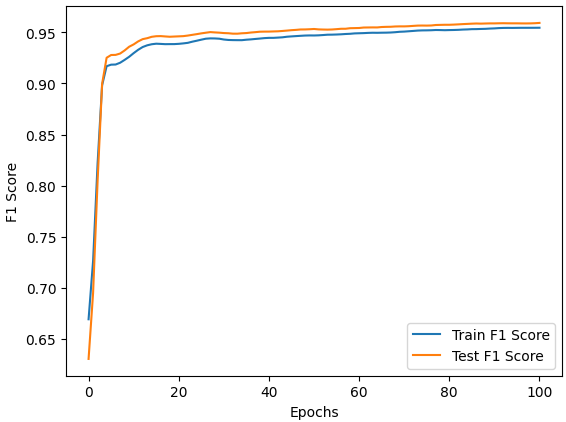
\includegraphics[width=\columnwidth]{F1-Epochs.png}
  \caption{Rate of change of weighted average F1 score with increasing number of epochs.}
  \label{fig:F1-Epochs}
\end{figure}

We used \texttt{Pytorch} to implement and train the model. The choice of the number of epochs was based on the rate of change of the F1 score,
which we observed in most cases to not significantly increase after 10 epochs, and plateau after 30 epochs. As shown in Figure~\ref{fig:F1-Epochs},
which is where we stopped.

\section{Results}
We have stayed true to the original paper and used the same train and test sets, indicated in Table~\ref{tab:Train-Test-Sets}, 
and have used the same evaluation metrics, indicated in Table~\ref{tab:Classification-Report}. For the sake of consistency, we have included
\textit{BC} in the test set, and all 8 books of \textit{BG} in the training set, even though it was not part of the original report.

\begin{table}[H]
  \centering
  \begin{tabular}{|l|c|c|}
  \hline
  \textbf{} & \textbf{Test Set} & \textbf{In or Out-of-domain} \\
  \hline
  Fold 1   & Piny & Out \\
  \hline
  Fold 2   & Ovid & Out \\
  \hline
  Fold 3   & Caesar & In \\
  \hline
  \end{tabular}
  \caption{Train and Test Sets for each fold}
  \label{tab:Train-Test-Sets}
\end{table}

To have a detailed overview of the results, we have included a classification report for each fold and each model 
in Table~\ref{tab:Classification-Report}, which includes the precision, recall, F1 score, and weighted average F1 score for each fold and each model,
namely Binary Clustering, Multi-Class Clustering, and Neural Network. While we understand that the standard score for NER is the
Span F1 score, we have used the normal F1 score for the sake of consistency with the original paper, as there is no mention of specificity of the type
of F1 score used, and we also understand that on a technical level we could not use the Span F1 score, as our model by design provides lower
performance than supervised models, so it was not in our final goal to achieve high scores measured by a more strict metric like Span F1.

\begin{table}[H]
  \centering
  \begin{tabular}{|l|c|c|c|c|}
  \hline
  \textbf{} & \textbf{Prec.} & \textbf{Rec.} & \textbf{M. F1} & \textbf{W. F1} \\
  \hline
  \multicolumn{5}{|c|}{\textit{Binary Clustering}} \\
  \hline
  Fold 1   & 0.90 & 0.91 & 0.91 & 0.99 \\
  Fold 2   & 0.86 & 0.78 & 0.82 & 0.98 \\
  Fold 3   & 0.98 & 0.98 & 0.98 & 1.00 \\
  \hline
  \multicolumn{5}{|c|}{\textit{Multi-Class Clustering}} \\
  \hline
  Fold 1   & 0.41 & 0.43 & 0.41 & 0.98 \\
  Fold 2   & 0.38 & 0.34 & 0.35 & 0.97 \\
  Fold 3   & 0.56 & 0.53 & 0.54 & 0.99 \\
  \hline
  \multicolumn{5}{|c|}{\textit{Neural Network}} \\
  \hline
  Fold 1   & 0.33 & 0.52 & 0.39 & 0.96 \\
  Fold 2   & 0.29 & 0.42 & 0.32 & 0.95 \\
  Fold 3   & 0.48 & 0.60 & 0.53 & 0.97 \\
  \hline
  \end{tabular}
  \caption{Classification report}
  \label{tab:Classification-Report}
\end{table}

These results suggest that binary clustering performs extraordinarily well, highly exceeding our expectations, however once we dive deeper
into being able to distinguish between different named entitities, the results also dive quite deep into the lower end of resulting scores.
Additionally, the Neural Network does not seem to provide substainal, if any at all, improvement over the multi-class clustering, however,
we must note that the purpose of the Neural Network is to generalise on unseen data, and not to specifically outperform the multi-class clustering.

There are a few key points worthy of mention, that may not be initially obvious.
Fold 3 represents the In Domain datasets, which have higher chance of performing better, as per our observation, the training and testing
datasets mention the same entities more often, resulting in a better fit. Finally, some entities are better detected, which the results table
also does not show. The entities that we found to be better detected, were GEO-B, GRP-B, PRS-B, with F1 scores on average of around 0.6 to 0.8
for each entity.

\section{Future Work}

As our results are not very promising, it gives us a glimpse into the mysteries of the Latin language, and the challenges of NER within it.
We plan to explore some aspects of this field as there is a lot of room for improvement, and a lot more to discover.

To start, we would like to explore having a much larger dataset to work with, and observe how results improve with the proportion of data.
Next, we would like to explore different capitalizations of the language, and observe how results change, as we
suspect that the capitalization played a significant role in the performance of the model.
Finally, considering an ensemble method of different models may prove to be the most effective approach, as it has been observed so far,
and we would like to explore the limits of this approach and benefits of it.

\section*{Limitations}

Due to the size of the dataset and the complexity of the task, we were not able to train a more capable model.
A similarly comparable evaluation of NER using an unsupervised model within the English language has been shown to achieve much better results,
indicating that the size and distribution of the dataset is a significant factor in the performance of the model, even more so than the choice of model.

Having a discrepancy between the original dataset wordcount and what we have received, based ont the original splits, having to
manually split the dataset has made our work substantially longer than expected, as we had to manually separate the dataset up into
new files. Using the help of the original source of the dataset, we managed to find and split it appropriately, at a significant cost of time.

Due to the limitations of time, we were not able to explore more methods of approach and tinker extensively with the hyperparameters of the model.

\bibliography{custom}

\begin{comment}
\newpage
\section*{.}
\newpage
\section{Introduction (Original)}
These instructions are for authors submitting papers to *ACL conferences using \LaTeX. They are not self-contained. All authors must follow the general instructions for *ACL proceedings,\footnote{\url{http://acl-org.github.io/ACLPUB/formatting.html}} and this document contains additional instructions for the \LaTeX{} style files.

The templates include the \LaTeX{} source of this document (\texttt{acl\_latex.tex}),
the \LaTeX{} style file used to format it (\texttt{acl.sty}),
an ACL bibliography style (\texttt{acl\_natbib.bst}),
an example bibliography (\texttt{custom.bib}),
and the bibliography for the ACL Anthology (\texttt{anthology.bib}).

\section{Engines}

To produce a PDF file, pdf\LaTeX{} is strongly recommended (over original \LaTeX{} plus dvips+ps2pdf or dvipdf).
The style file \texttt{acl.sty} can also be used with
lua\LaTeX{} and
Xe\LaTeX{}, which are especially suitable for text in non-Latin scripts.
The file \texttt{acl\_lualatex.tex} in this repository provides
an example of how to use \texttt{acl.sty} with either
lua\LaTeX{} or
Xe\LaTeX{}.

\section{Preamble}

The first line of the file must be
\begin{quote}
\begin{verbatim}
\documentclass[11pt]{article}
\end{verbatim}
\end{quote}

To load the style file in the review version:
\begin{quote}
\begin{verbatim}
\usepackage[review]{acl}
\end{verbatim}
\end{quote}
For the final version, omit the \verb|review| option:
\begin{quote}
\begin{verbatim}
\usepackage{acl}
\end{verbatim}
\end{quote}

To use Times Roman, put the following in the preamble:
\begin{quote}
\begin{verbatim}
\usepackage{times}
\end{verbatim}
\end{quote}
(Alternatives like txfonts or newtx are also acceptable.)

Please see the \LaTeX{} source of this document for comments on other packages that may be useful.

Set the title and author using \verb|\title| and \verb|\author|. Within the author list, format multiple authors using \verb|\and| and \verb|\And| and \verb|\AND|; please see the \LaTeX{} source for examples.

By default, the box containing the title and author names is set to the minimum of 5 cm. If you need more space, include the following in the preamble:
\begin{quote}
\begin{verbatim}
\setlength\titlebox{<dim>}
\end{verbatim}
\end{quote}
where \verb|<dim>| is replaced with a length. Do not set this length smaller than 5 cm.

\section{Document Body}

\subsection{Footnotes}

Footnotes are inserted with the \verb|\footnote| command.\footnote{This is a footnote.}

\subsection{Tables and figures}

See Table~\ref{tab:accents} for an example of a table and its caption.
\textbf{Do not override the default caption sizes.}

\begin{table}
  \centering
  \begin{tabular}{lc}
    \hline
    \textbf{Command} & \textbf{Output} \\
    \hline
    \verb|{\"a}|     & {\"a}           \\
    \verb|{\^e}|     & {\^e}           \\
    \verb|{\`i}|     & {\`i}           \\
    \verb|{\.I}|     & {\.I}           \\
    \verb|{\o}|      & {\o}            \\
    \verb|{\'u}|     & {\'u}           \\
    \verb|{\aa}|     & {\aa}           \\\hline
  \end{tabular}
  \begin{tabular}{lc}
    \hline
    \textbf{Command} & \textbf{Output} \\
    \hline
    \verb|{\c c}|    & {\c c}          \\
    \verb|{\u g}|    & {\u g}          \\
    \verb|{\l}|      & {\l}            \\
    \verb|{\~n}|     & {\~n}           \\
    \verb|{\H o}|    & {\H o}          \\
    \verb|{\v r}|    & {\v r}          \\
    \verb|{\ss}|     & {\ss}           \\
    \hline
  \end{tabular}
  \caption{Example commands for accented characters, to be used in, \emph{e.g.}, Bib\TeX{} entries.}
  \label{tab:accents}
\end{table}

As much as possible, fonts in figures should conform
to the document fonts. See Figure~\ref{fig:experiments} for an example of a figure and its caption.

Using the \verb|graphicx| package graphics files can be included within figure
environment at an appropriate point within the text.
The \verb|graphicx| package supports various optional arguments to control the
appearance of the figure.
You must include it explicitly in the \LaTeX{} preamble (after the
\verb|\documentclass| declaration and before \verb|\begin{document}|) using
\verb|\usepackage{graphicx}|.

\begin{figure}[t]
  \includegraphics[width=\columnwidth]{example-image-golden}
  \caption{A figure with a caption that runs for more than one line.
    Example image is usually available through the \texttt{mwe} package
    without even mentioning it in the preamble.}
  \label{fig:experiments}
\end{figure}

\begin{figure*}[t]
  \includegraphics[width=0.48\linewidth]{example-image-a} \hfill
  \includegraphics[width=0.48\linewidth]{example-image-b}
  \caption {A minimal working example to demonstrate how to place
    two images side-by-side.}
\end{figure*}

\subsection{Hyperlinks}

Users of older versions of \LaTeX{} may encounter the following error during compilation:
\begin{quote}
\verb|\pdfendlink| ended up in different nesting level than \verb|\pdfstartlink|.
\end{quote}
This happens when pdf\LaTeX{} is used and a citation splits across a page boundary. The best way to fix this is to upgrade \LaTeX{} to 2018-12-01 or later.

\subsection{Citations}

\begin{table*}
  \centering
  \begin{tabular}{lll}
    \hline
    \textbf{Output}           & \textbf{natbib command} & \textbf{ACL only command} \\
    \hline
    \citep{Gusfield:97}       & \verb|\citep|           &                           \\
    \citealp{Gusfield:97}     & \verb|\citealp|         &                           \\
    \citet{Gusfield:97}       & \verb|\citet|           &                           \\
    \citeyearpar{Gusfield:97} & \verb|\citeyearpar|     &                           \\
    \citeposs{Gusfield:97}    &                         & \verb|\citeposs|          \\
    \hline
  \end{tabular}
  \caption{\label{citation-guide}
    Citation commands supported by the style file.
    The style is based on the natbib package and supports all natbib citation commands.
    It also supports commands defined in previous ACL style files for compatibility.
  }
\end{table*}

Table~\ref{citation-guide} shows the syntax supported by the style files.
We encourage you to use the natbib styles.
You can use the command \verb|\citet| (cite in text) to get ``author (year)'' citations, like this citation to a paper by \citet{Gusfield:97}.
You can use the command \verb|\citep| (cite in parentheses) to get ``(author, year)'' citations \citep{Gusfield:97}.
You can use the command \verb|\citealp| (alternative cite without parentheses) to get ``author, year'' citations, which is useful for using citations within parentheses (e.g. \citealp{Gusfield:97}).

A possessive citation can be made with the command \verb|\citeposs|.
This is not a standard natbib command, so it is generally not compatible
with other style files.


\subsection{References}

\nocite{Ando2005,andrew2007scalable,rasooli-tetrault-2015}

The \LaTeX{} and Bib\TeX{} style files provided roughly follow the American Psychological Association format.
If your own bib file is named \texttt{custom.bib}, then placing the following before any appendices in your \LaTeX{} file will generate the references section for you:
\begin{quote}
\begin{verbatim}
\bibliography{custom}
\end{verbatim}
\end{quote}

You can obtain the complete ACL Anthology as a Bib\TeX{} file from \url{https://aclweb.org/anthology/anthology.bib.gz}.
To include both the Anthology and your own .bib file, use the following instead of the above.
\begin{quote}
\begin{verbatim}
\bibliography{anthology,custom}
\end{verbatim}
\end{quote}

Please see Section~\ref{sec:bibtex} for information on preparing Bib\TeX{} files.

\subsection{Equations}

An example equation is shown below:
\begin{equation}
  \label{eq:example}
  A = \pi r^2
\end{equation}

Labels for equation numbers, sections, subsections, figures and tables
are all defined with the \verb|\label{label}| command and cross references
to them are made with the \verb|\ref{label}| command.

This an example cross-reference to Equation~\ref{eq:example}.

\subsection{Appendices}

Use \verb|\appendix| before any appendix section to switch the section numbering over to letters. See Appendix~\ref{sec:appendix} for an example.

\section{Bib\TeX{} Files}
\label{sec:bibtex}

Unicode cannot be used in Bib\TeX{} entries, and some ways of typing special characters can disrupt Bib\TeX's alphabetization. The recommended way of typing special characters is shown in Table~\ref{tab:accents}.

Please ensure that Bib\TeX{} records contain DOIs or URLs when possible, and for all the ACL materials that you reference.
Use the \verb|doi| field for DOIs and the \verb|url| field for URLs.
If a Bib\TeX{} entry has a URL or DOI field, the paper title in the references section will appear as a hyperlink to the paper, using the hyperref \LaTeX{} package.


\section*{Limitations}

Since December 2023, a "Limitations" section has been required for all papers submitted to ACL Rolling Review (ARR). This section should be placed at the end of the paper, before the references. The "Limitations" section (along with, optionally, a section for ethical considerations) may be up to one page and will not count toward the final page limit. Note that these files may be used by venues that do not rely on ARR so it is recommended to verify the requirement of a "Limitations" section and other criteria with the venue in question.

\section*{Acknowledgments}

This document has been adapted
by Steven Bethard, Ryan Cotterell and Rui Yan
from the instructions for earlier ACL and NAACL proceedings, including those for
ACL 2019 by Douwe Kiela and Ivan Vuli\'{c},
NAACL 2019 by Stephanie Lukin and Alla Roskovskaya,
ACL 2018 by Shay Cohen, Kevin Gimpel, and Wei Lu,
NAACL 2018 by Margaret Mitchell and Stephanie Lukin,
Bib\TeX{} suggestions for (NA)ACL 2017/2018 from Jason Eisner,
ACL 2017 by Dan Gildea and Min-Yen Kan,
NAACL 2017 by Margaret Mitchell,
ACL 2012 by Maggie Li and Michael White,
ACL 2010 by Jing-Shin Chang and Philipp Koehn,
ACL 2008 by Johanna D. Moore, Simone Teufel, James Allan, and Sadaoki Furui,
ACL 2005 by Hwee Tou Ng and Kemal Oflazer,
ACL 2002 by Eugene Charniak and Dekang Lin,
and earlier ACL and EACL formats written by several people, including
John Chen, Henry S. Thompson and Donald Walker.
Additional elements were taken from the formatting instructions of the \emph{International Joint Conference on Artificial Intelligence} and the \emph{Conference on Computer Vision and Pattern Recognition}.

% Bibliography entries for the entire Anthology, followed by custom entries
%\bibliography{anthology,custom}
% Custom bibliography entries only
\bibliography{custom}

\appendix

\section{Example Appendix}
\label{sec:appendix}

This is an appendix.
\end{comment}

\end{document}
